\documentclass[border=8pt]{standalone}
\usepackage{fontspec}
\setsansfont{Arial}
\usepackage{pgfplots}
\pgfplotsset{compat=1.18,
  every axis/.append style={/pgf/number format/assume math mode=true,
    tick label style={font=\sffamily\small},
    nodes near coords style={font=\sffamily\scriptsize}}}
% Validation AP@[.50:.95] (%) of the T41 search and confirmation runs.
% Source: docs/t41-handoff.md, training-only completion record (PR #25).
\begin{document}
\sffamily\small
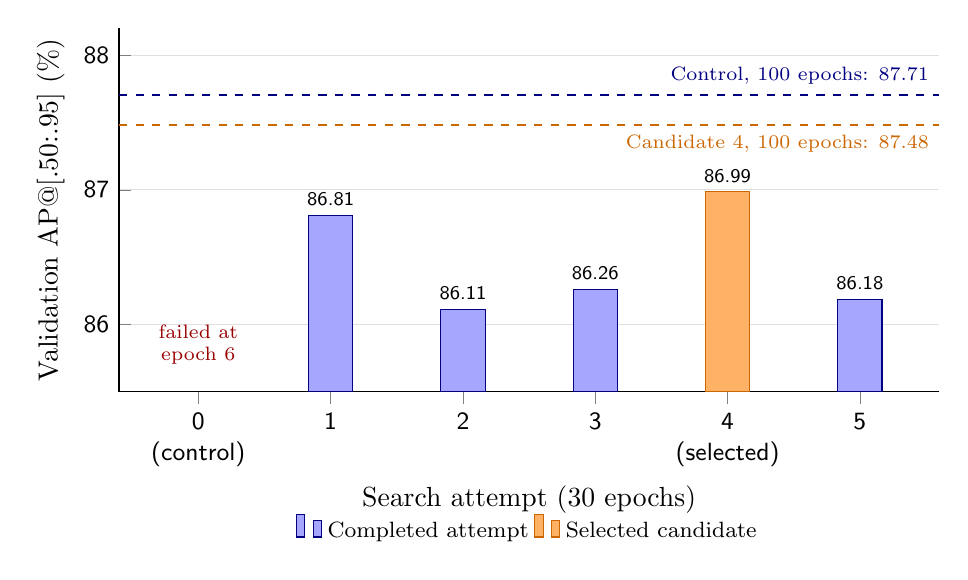
\begin{tikzpicture}
\begin{axis}[
  width=12cm,height=6.2cm,
  ybar,bar width=16pt,
  ymin=85.5,ymax=88.2,
  ylabel={Validation AP@[.50:.95] (\%)},
  xlabel={Search attempt (30 epochs)},
  xtick={0,1,2,3,4,5},
  xticklabels={0\\(control),1,2,3,4\\(selected),5},
  xticklabel style={align=center},
  xmin=-0.6,xmax=5.6,
  nodes near coords,
  nodes near coords style={/pgf/number format/.cd,fixed,fixed zerofill,precision=2},
  ymajorgrids,grid style={black!12},
  axis lines*=left,
  legend style={font=\footnotesize,draw=none,fill=none,at={(0.5,-0.32)},anchor=north,legend columns=-1},
  legend cell align=left,
]
\addplot[fill=blue!35,draw=blue!50!black,bar shift=0pt] coordinates
  {(1,86.811) (2,86.113) (3,86.262) (5,86.184)};
\addplot[fill=orange!60,draw=orange!80!black,bar shift=0pt] coordinates {(4,86.985)};
\draw[blue!50!black,thick,dashed] (axis cs:-0.6,87.706) -- (axis cs:5.6,87.706)
  node[pos=1,above left,font=\scriptsize] {Control, 100 epochs: 87.71};
\draw[orange!80!black,thick,dashed] (axis cs:-0.6,87.483) -- (axis cs:5.6,87.483)
  node[pos=1,below left,font=\scriptsize] {Candidate 4, 100 epochs: 87.48};
\node[font=\scriptsize,text=red!60!black,align=center] at (axis cs:0,85.85) {failed at\\epoch 6};
\legend{Completed attempt,Selected candidate}
\end{axis}
\end{tikzpicture}
\end{document}
